\documentclass{article}
\usepackage{graphicx}
\usepackage{amsmath}


\title{TP1 ADM}
\author{MARIAC Damien, Matteo Scaia}
\date{\today} 

\begin{document}

\maketitle

\begin{figure}[h] 
    \centering
    
\includegraphics[width=0.5\textwidth]{ssd_logo.png} 
\end{figure}

\newpage
\tableofcontents
\newpage

\section{Introduction}
On dispose d'un jeu de donnees présentant une étude de 27 espèces d'arbres dans 1000 parcelles d'une forêt.
Il s'agit d'étudier la variabilité des densités de peuplement d'espèces arborées dans différentes parcelles de la forêt du bassin du Congo.
Nous disposons dans notre jeu de donnée 30 variables quantitatives dont : 27 variables de comptage des espèces, la surface de la parcelle, 2 variables une forestier et une géologique.
Et une variable qualitative "code".

\section{Partie 1}
\subsection{inertie et barycentre}

Nous cherchons à calculer la densité de peuplement de chaque espece par unité de surface. Nous calculons alors pour chaque parcelle:
\[
(d_j^i)_{1 \leq j \leq 1000}^{1 \leq i \leq 27} = \frac{x_j^i}{s_j}
\]

\begin{table}[h]
    \centering
    \caption{Extrait de densité}
    \label{tab:donnees_extrait}
    \begin{tabular}{|c|c|c|c|c|}
    \hline
    \textbf{Code} & \textbf{Gen1} & \textbf{Gen5} & \textbf{Gen10}\\
    \hline
    1 & 0 & 0 & 2.200 \\
    2 & 0.6 & 0.133 & 1.333  \\
    3 & 0.514 & 0.057 & 3.6 \\
    4 & 0 & 0.439 & 0.244 \\
    5 & 0.095 & 0 & 0.476 \\
    \hline
    \end{tabular}
    \end{table}


Nous utiliserons des densités plutôt que des comptages car cela permet de normaliser les données par rapport à la taille de la parcelle,
ce qui rend les comparaisons entre les parcelles équitables.
\\
Nous devons centrer et reduire les variables quantitatives dans le but de mieux comparer celles qui decrivent les différents densité.
Nous allons alors utiliser :
\[
(x_j^i)_{1 \leq i \leq 27} = \frac{x_j^i - \bar{x}_j}{\sigma_j}
\]

Avec $\bar{x}_j$ la moyenne pour la j eme variable et  $\sigma_j$ l'ecart-type de la variable quantitative j.
\\
\\
\textbf{Par consequents on a:}
\\
\\
\underline{Barycentre à l'origine :} (preuve théorique)
\\

Supposons que nous avons un ensemble de données $X$ composé de $n$ observations et $p$ variables. Après le centrage et la réduction, la matrice transformée $X'$ est définie par :

\[
\tilde{x}_{ij} = \frac{x_{ij} - \overline{x}_j}{s_j}
\]

où $\overline{x}_j$ est la moyenne et $s_j$ l'écart-type de la $j$-ème variable.


Le barycentre de $X$ est donné par la moyenne de chaque colonne de $X$. Calculons cette moyenne pour n'importe quelle j:

\[
\overline{x}_j = \frac{1}{n} \sum_{i=1}^n \tilde{x}_{ij} = \frac{1}{n} \sum_{i=1}^n \frac{x_{ij} - \overline{x}_j}{s_j} = \frac{1}{s_j} \left(\frac{1}{n} \sum_{i=1}^n x_{ij}\right) - \frac{\overline{x}_j}{s_j} = 0
\]

Ainsi, le barycentre de chaque variable dans $X'$ est zéro.
\\
\\

\underline{Inertie totale égale à 27 :} (preuve théorique)
\\
\\
Considérons la meme matrice de données $X$. Après centrage et réduction, chaque élément de la matrice transformée $X'$ est défini par:
\[
x'_{ij} = \frac{x_{ij} - \overline{x}_j}{s_j}
\]

En reprenant les mêmes notations que avant.


L'inertie de l'ensemble des points $X'$ par rapport à leur barycentre $\mathbf{y}_M$ est définie par:
\[
I_{Y, W} = \sum_{i=1}^n w_i \|\mathbf{x}_i - \mathbf{y}\|^2
\]

Pour les données centrées-réduites, chaque $\mathbf{x}_i'$ est déjà centré, donc le barycentre $\mathbf{y} = \mathbf{0}$. Par conséquent, la formule de l'inertie se simplifie à:
\[
I_{Y, W} = \sum_{i=1}^n w_i \|\mathbf{x}_i'\|^2
\]

Si tous les poids $w_i$ sont égaux (par exemple, $w_i = \frac{1}{n}$ ce qui est notre cas), alors l'inertie devient:
\[
I_{Y, W} = \frac{1}{n} \sum_{i=1}^n \|\mathbf{x}_i'\|^2
\]

Comme chaque $\mathbf{x}_i'$ est une observation centrée-réduite et la variance de chaque variable est 1, nous avons (pour i fixé):
\[
\|\mathbf{x}_i'\|^2 = \sum_{j=1}^p (x'_{ij})^2 = p
\]

Ainsi, l'inertie totale est:
\[
I_{Y, W} = \frac{1}{n} \sum_{i=1}^n p = p 
\]
ce qui montre que l'inertie totale du nuage des données centrées-réduites est égale au nombre de variables $p$ (qui dans notre cas vaut 27).

\subsection{Autour des types forestiers}

Dans cette section, nous calculons les barycentres des sept types forestiers présents dans les données, ainsi que l'inertie inter-types et le coefficient $R^2$ associé à la partition des parcelles selon ces types. Ce calcul nous permet d'évaluer la proportion de la variabilité totale des densités de peuplement expliquée par cette partition.

\subsubsection{Calcul des poids des types forestiers}
Le poids de chaque type forestier est calculé comme la proportion de parcelles appartenant à ce type par rapport à l'ensemble des 1000 parcelles. C'est à dire, le poids est donné par :

\[
p_i = \frac{\text{Nombre de parcelles du type } i}{1000}
\]


\subsubsection{Calcul des barycentres des types forestiers}
Pour chaque type forestier, si on note $X$ la matrice des densités standardisées (matrice $1000 \times 27$), alors le barycentre vaut :

\[
\bar{X}_i = \frac{1}{n_i} \sum_{j \in \text{Type } i} X_j
\]

Cela nous donne comme tableau :

\begin{figure}[h] 
    \centering
    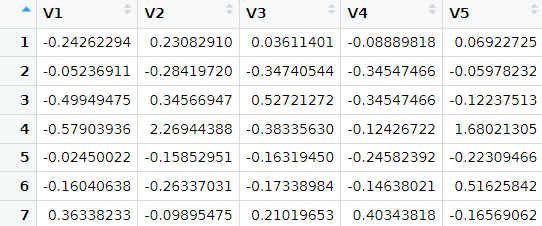
\includegraphics[width=0.5\textwidth]{barycentre_forestier.png} 
\end{figure}


\subsubsection{Calcul des normes euclidiennes carrées}
Une fois les barycentres calculés, nous évaluons la distance de chaque barycentre à l'origine de l'espace des 27 densités centré reduite. La distance est induite par la norme 2 et donc :
Ce qui nous donne comme extrait de tableau : 

\[
\|\bar{X}_i\|^2 = \sum_{k=1}^{27} \bar{X}_{i,k}^2
\]

Ces normes euclidiennes carrées sont calculées pour chaque type forestier.

\subsection{Inertie inter-types et coefficient $R^2$}
L'inertie inter-types forestiers est calculée en pondérant les normes euclidiennes carrées par les poids des types forestiers. Elle mesure la variabilité des densités de peuplement expliquée par la partition en types forestiers et est définie par :

\[
\text{Inertie inter-types} = \sum_{i=1}^{7} p_i \|\bar{X}_i\|^2
\]

Le coefficient $R^2$, qui exprime la proportion de la variabilité totale des densités de peuplement expliquée par cette partition, est donné par le rapport entre l'inertie inter-types et l'inertie totale (27, correspondant au nombre de variables). Il est donc calculé par :

\[
R^2 = \frac{\text{Inertie inter-types}}{\text{Inertie totale}}
\]

Ce coefficient $R^2$ nous permet d'évaluer dans quelle mesure les types forestiers expliquent la variabilité des densités de peuplement dans les parcelles observées.



\newpage
\section{Conclusion}

\end{document}
